\chapter{Methodology}

This chapter explains how we ran the experiments: first an overview of the design, then model architecture, datasets, training setup with tuning, and the evaluation protocol. We favor simple choices that are easy to reproduce. When trade‑offs appear, we keep the setup stable—deliberately straightforward by design.

\section{Experimental Design Overview}

We evaluate \textbf{10 pretraining configurations}: 2 mixtures (Financial; Wiki+Financial) and 8 single dataset baselines. Each configuration is trained at three model sizes (0.6B/1.7B/4B) with a fixed \textbf{100M token budget} and evaluated on \textbf{8 held out test sets}. We also run 6 follow up runs with adjusted learning rates to address training stability at larger scales. We kept other factors fixed where possible. \Cref{tab:exp_settings} summarizes the settings used throughout.

% Experimental Settings Summary Table
\begin{table}[h]
\centering
\caption[Experimental Settings Summary]{Summary of experimental settings used across all pretraining runs.}
\label{tab:exp_settings}
\small
\begin{tabular}{p{3.8cm} p{9.5cm}}
\toprule
\textbf{Aspect} & \textbf{Setting} \\
\midrule
Pretraining configurations & 10 total: 2 mixtures (Financial; Wiki+Financial) + 8 single-dataset runs \\
Model sizes & Qwen3-0.6B, Qwen3-1.7B, Qwen3-4B \\
Token budget & 100M tokens per run (normalized across datasets and model sizes) \\
Sequence length & 1{,}024 tokens \\
Optimizer & AdamW ($\beta_1$=0.9, $\beta_2$=0.999, $\epsilon$=$10^{-8}$), weight decay 0.01 \\
LR schedule & Cosine decay, 1{,}000 warmup steps, minimum LR $10^{-6}$ \\
Learning rate & $2\times10^{-5}$ for all main runs; ad-hoc smaller LRs used in a few follow-ups when anomalies were observed \\
Batching & Effective batch size 8; gradient accumulation used only when memory was insufficient \\
Precision & bfloat16 mixed precision; dropout 0.0 \\
Hardware & NVIDIA RTX A6000 (48GB), A100 (40GB), H100 (80GB); GPUs rented from Lambda Labs \\
Mixture policy & 50cap-proportional sampling (sampling cap; does not change corpus sizes) to limit dominance of large sources \\
Evaluation & 8 held-out test sets (7 financial + WikiText); metrics: Cross-Entropy, Perplexity, Relative Spread\% \\
\bottomrule
\end{tabular}
\end{table}


This design supports our research questions on mixture composition, model scale, dataset size, and domain transfer. Results appear in Chapter 4 with figures and tables. We report measurements; we avoid theory claims.

\section{Model Architecture}

We use the \textbf{Qwen3 model family} \parencite{yang2024qwen2,qwen3}, a series of open source transformer based decoder only language models pretrained on diverse multilingual corpora. Qwen3 employs grouped query attention (GQA) for memory efficiency and supports both standard and flash attention. We select three sizes from the Qwen3 Base series (pretrained checkpoints without post training alignment), detailed in \Cref{tab:model_specs}. In our runs, these sizes allow clean comparisons without changing tokenizers or context limits.

\begin{table}[h]
\centering
\caption[Qwen3 Model Specifications]{Qwen3 model specifications across three scales. All models use the same tokenizer (151,643 tokens) and support 32K context length. Training memory shown for bfloat16 precision.}
\label{tab:model_specs}
\begin{tabular}{lcccccc}
\toprule
\textbf{Model} & \textbf{Parameters} & \textbf{Layers} & \textbf{Hidden} & \textbf{Heads} & \textbf{GQA} & \textbf{Memory} \\
\midrule
Qwen3-0.6B & 600M & 16 & 1024 & 16 & 4 & $\sim$4GB \\
Qwen3-1.7B & 1.7B & 24 & 2048 & 16 & 4 & $\sim$10GB \\
Qwen3-4B & 4.0B & 40 & 2560 & 20 & 4 & $\sim$20GB \\
\bottomrule
\end{tabular}
\end{table}

We chose Qwen3 for three reasons: (1) architectural consistency across scales enables clean size comparisons, (2) stable baseline performance on general and domain‑specific benchmarks, and (3) efficient inference suitable for edge deployment (all models fit on consumer hardware). Stated differently, it lets us study scale without changing too many other factors and reduces engineering noise.

\section{Datasets}

\subsection{Financial Datasets}

We curate 7 financial datasets spanning diverse tasks, document types, and data scales (total: 321.4M tokens), summarized in \Cref{tab:financial_datasets}. These datasets vary in size (0.3M to 197M tokens), format (news, reports, Q\&A, social media), and formality (regulatory filings vs tweets). This diversity lets us examine intra domain effects without changing models.

\begin{table}[h]
\centering
\caption[Financial Dataset Characteristics]{Financial dataset characteristics. Total: 321.4M tokens across 7 datasets with diverse genres and scales.}
\label{tab:financial_datasets}
\small
\begin{tabular}{p{3cm}cccp{5.5cm}}
\toprule
\textbf{Dataset} & \textbf{Examples} & \textbf{Tokens} & \textbf{Genre} & \textbf{Description} \\
\midrule
Lettria Financial News & 300K & 197M & Journalism & Long-form articles on markets, earnings, policy \\
\midrule
SEC Financial Reports & 54.3K & 80M & Regulatory & 10-K/10-Q excerpts with formal disclosures, legal language \\
\midrule
FinGPT Sentiment & 76.8K & 19.1M & Instruction & Headlines + sentiment labels in conversational format \\
\midrule
Finance Alpaca & 68.9K & 17.2M & Q\&A & Instruction-response pairs on financial concepts \\
\midrule
FiQA & 17.4K & 4.3M & Forum & User-generated Q\&A from forums and microblogs \\
\midrule
Financial QA 10K & 7.1K & 3.5M & Document & Questions on 10-K filings requiring tabular reasoning \\
\midrule
Twitter Sentiment & 1.1K & 0.3M & Social Media & Labeled tweets ($<$280 chars) with informal language \\
\bottomrule
\end{tabular}
\end{table}

\subsection{WikiText}

We use \textbf{WikiText 103} \parencite{merity2016pointer} as a general domain baseline, summarized in \Cref{tab:wikitext_dataset}. WikiText serves two purposes: (1) evaluating domain transfer (general $\leftrightarrow$ financial), and (2) testing whether high quality general corpora complement financial pretraining in mixtures. Sometimes it helps; sometimes not.

\begin{table}[h]
\centering
\caption[WikiText Dataset Characteristics]{WikiText-103 characteristics. Similar scale to SEC; smaller than News.}
\label{tab:wikitext_dataset}
\small
\begin{tabular}{p{3cm}cccp{5.5cm}}
\toprule
\textbf{Dataset} & \textbf{Examples} & \textbf{Tokens} & \textbf{Genre} & \textbf{Description} \\
\midrule
WikiText-103 & 103K & 103M & Encyclopedia & Verified Wikipedia articles with formal register, broad topical coverage, clean preprocessing \\
\bottomrule
\end{tabular}
\end{table}

\subsection{Mixture Strategies}

We employ a \textbf{50\% capping strategy} (``50cap'') for dataset mixing to balance diversity with data efficiency. The algorithm works as follows:

\textbf{Step 1 - Cap dominant datasets}: Identify the largest dataset in the mixture. If its token count exceeds 50\% of the total mixture, cap it at exactly 50\%. This prevents any single dataset from dominating the mixture.

\textbf{Step 2 - Proportional sampling}: For remaining datasets (below 50\% threshold), sample tokens proportionally to their original sizes. This preserves relative contributions while ensuring diversity.

\textbf{Step 3 - Token-level interleaving}: During training, sample batches from the mixed distribution at the token level (not example level). This ensures fine-grained mixing throughout training rather than sequential block exposure.

\textbf{Example}: For the 7‑dataset financial mixture (News 197M, SEC 80M, FinGPT 19M, Alpaca 17M, FiQA 4M, Financial QA 3.5M, Twitter 0.3M; total 321M tokens), News exceeds 50\% (61.4\%) and is capped at 50\% (160.5M tokens); the remaining datasets are sampled proportionally from the other 160.5M‑token budget; the final mixture stays at $\sim$321M tokens with News contributing exactly half.

\begin{figure}[h]
\centering
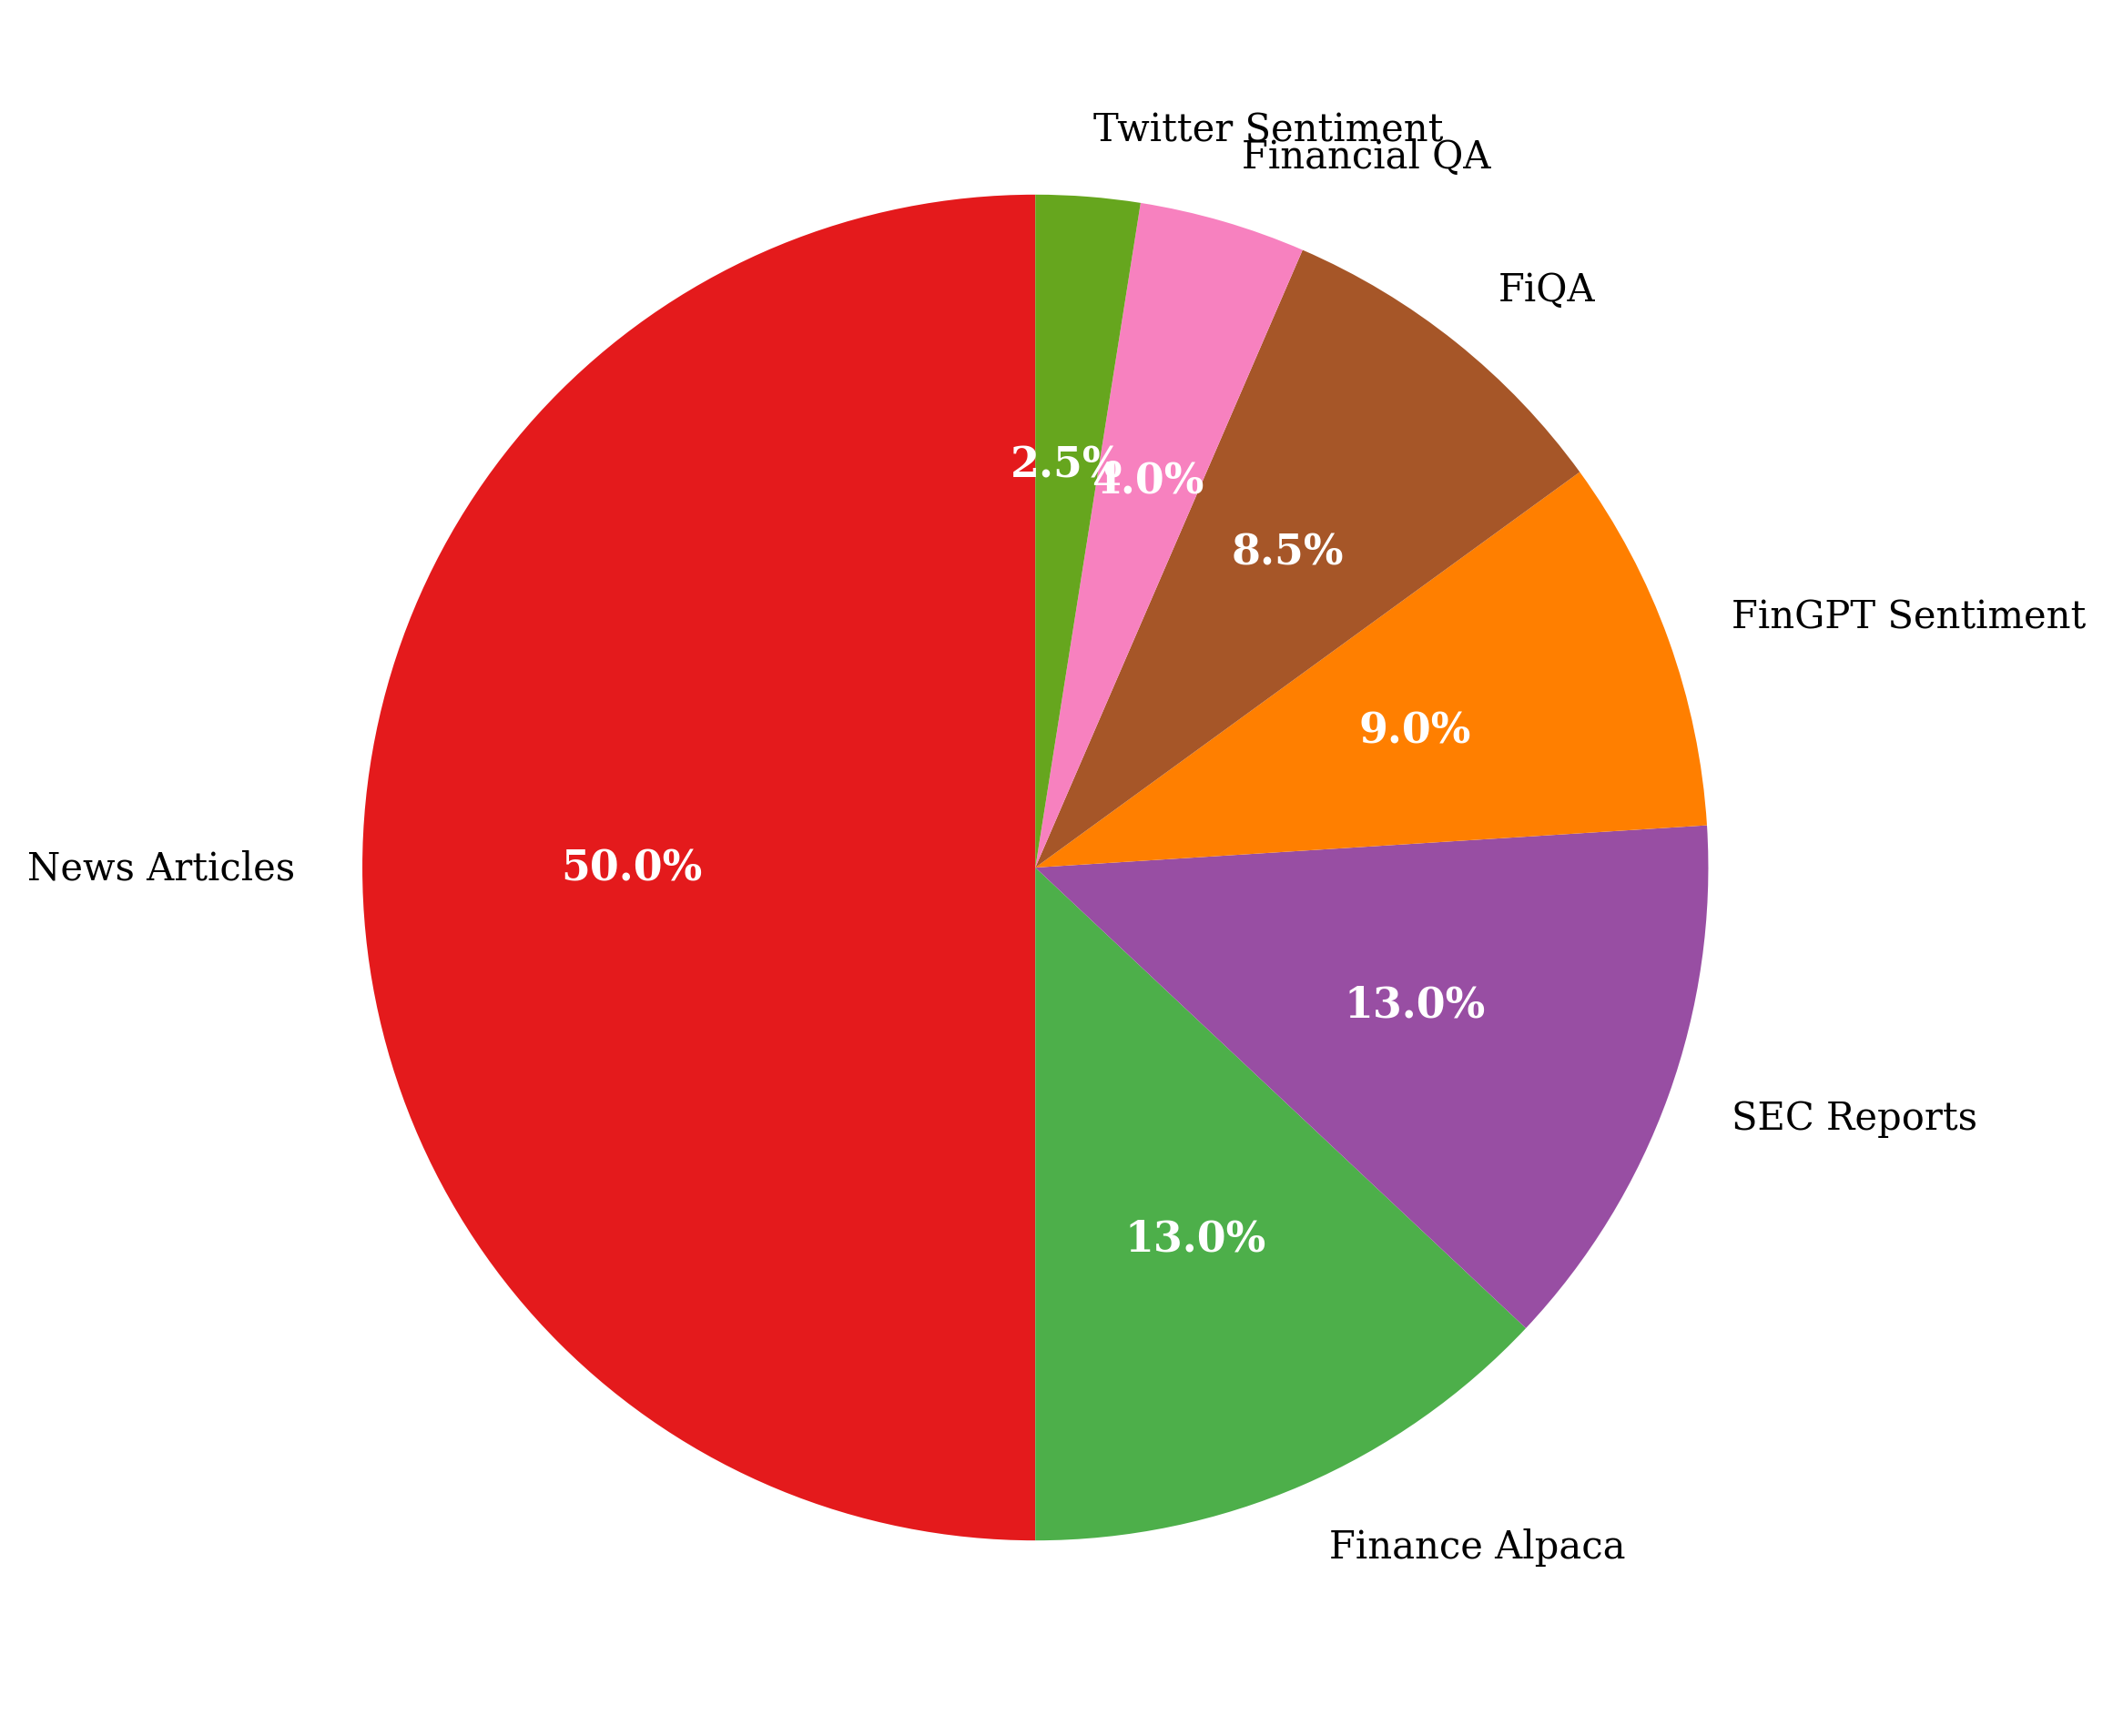
\includegraphics[width=0.95\textwidth]{figures/diagram_50cap.png}
\caption[50cap Mixture Strategy Visualization]{Token allocation in Mixed Financial dataset using 50cap strategy. News Articles is capped to contribute at most 50\% in sampling (illustrative normalization; raw corpus remains 197M). The remaining six datasets are sampled proportionally from the other 50\%, ensuring diversity while preventing dominance. Left panel shows pie chart view; right panel shows stacked bar view with total allocation.}
\label{fig:diagram_50cap}
\end{figure}

\Cref{fig:diagram_50cap} visualizes the 50cap sampling policy: News Articles (red) is capped to at most 50\% of sampled tokens; the remaining 50\% is distributed proportionally among the other six datasets. The pie (left) shows percentage composition; the stacked bar (right) normalizes absolute counts to a 50/50 split (\(\approx\!160.7\,\text{M}+\approx\!160.7\,\text{M}\) if scaled to the 321.4M corpus total) for illustration only — 50cap does not modify raw corpus sizes.

For the 8-dataset WikiText+Financial mixture, WikiText (100M) and News (197M) are both large; we apply 50cap to ensure neither dominates, then proportionally sample the other 6 financial datasets.

This strategy contrasts with temperature sampling (which requires tuning hyperparameters) and equal mixing (which severely undersamples large datasets). The 50cap approach is deterministic, requires no tuning, and empirically performs well in production settings \parencite{longpre2023pretrainer}.

\section{Training Setup and Hyperparameter Tuning}

\subsection{Initial Configuration}

We trained all models with a single hyperparameter template to set a baseline. Standard causal LM choices:

\textbf{Optimizer}: AdamW with $\beta_1=0.9$, $\beta_2=0.999$, $\epsilon=10^{-8}$, weight decay $0.01$

\textbf{Learning Rate}: $2 \times 10^{-5}$ (used for all main settings)

\textbf{LR Schedule}: Cosine decay with 1,000 warmup steps, minimum LR $10^{-6}$

\textbf{Batch Configuration}: Effective batch size 8 across all runs. When memory was tight, we used gradient accumulation to keep the same effective batch size.

\textbf{Sequence Length}: 1,024 tokens (fixed for all runs)

\textbf{Precision}: bfloat16 mixed precision for memory efficiency

\textbf{Training Duration}: Dataset-dependent. Small datasets ($<$20K samples) trained for maximum epochs to reach $\sim$100M token budget; large datasets trained for 2-5 epochs. All models exposed to approximately 100M training tokens for fair comparison.

\textbf{Hardware}: NVIDIA RTX A6000 (48GB), A100 (40GB), and H100 (80GB) GPUs rented from Lambda Labs. Gradient accumulation was applied as needed to fit memory constraints.

When we observed abnormalities in a few experiments, we reran those specific cases with smaller LRs as a simple heuristic to stabilize training. We do not claim any theoretical scaling rule for LR; these adjustments were pragmatic.

\subsection{Pragmatic Learning Rate Adjustments}

In three configurations we observed abnormal behavior (e.g., larger models underperforming smaller ones). For these few cases, we retried with smaller learning rates (e.g., $1\times 10^{-5}$ or $5\times 10^{-6}$) purely as a practical heuristic to stabilize training. We do not propose or rely on a learning-rate scaling theory in this work. LR-comparison tables for the affected settings are reported in Chapter~4.

\subsection{Other Hyperparameters}

Beyond learning rate, we maintained consistent hyperparameters across experiments:

\textbf{Batch Size and Accumulation}: Effective batch size 8 across all runs. We used gradient accumulation only when necessary to fit models and sequence lengths into GPU memory.

\textbf{Warmup Steps}: 1,000 steps (3.1\% of training for 32K total steps) provided sufficient stabilization during initial training. Longer warmup did not improve final performance.

\textbf{Training Epochs}: Varied by dataset size to normalize token exposure. Small datasets (Twitter, Financial QA) trained for 67-249 epochs to reach 100M token budget; medium datasets (FiQA, FinGPT, Alpaca) for 6-30 epochs; large datasets (SEC, News) for 2-24 epochs. This normalization ensures fair comparison across datasets of different sizes.

\textbf{Maximum Sequence Length}: 1,024 tokens. Financial documents often exceed this length (SEC filings: 10K+ tokens), but longer sequences quadratically increase memory and slow training. We accept truncation as a practical trade-off.

\textbf{Dropout}: 0.0 (no dropout) following common practice for large-scale pretraining where overfitting is rarely observed.

\subsection{Computational Budget}

To ensure fair comparison across experiments, we normalized the token budget to \textbf{100M tokens per training run}, regardless of dataset size or model scale. This design controls for data exposure while allowing investigation of how model size and data characteristics interact. A simple rule that kept the study manageable.

\textbf{Experimental Scale}: In total we ran 36 trainings: two mixture settings (Mixed Financial; Mixed Wiki+Financial), eight single‑dataset baselines (WikiText, Financial News, SEC, FinGPT, Finance Alpaca, FiQA, Financial QA 10K, Twitter), each at three sizes (0.6B/1.7B/4B) for 30 baselines, plus six follow‑ups with reduced learning rates on the three problematic datasets (WikiText, Financial QA, Twitter) to probe sensitivity at larger scales.

\textbf{Total computational cost}: $36 \times 100\text{M} = 3.6\text{B}$ tokens processed. On a single NVIDIA A100 (40GB) rented from Lambda Labs, each 100M-token run required 2 to 8 hours depending on model size (0.6B: $\sim$2h, 1.7B: $\sim$4h, 4B: $\sim$8h), totaling approximately 150 GPU-hours for the complete experimental suite.

This token controlled design helps ensure that performance differences reflect model data interactions rather than unequal training compute. Variable epoch counts (2 to 249 across experiments) follow from dataset size while keeping token exposure constant. But it also means small datasets see many passes. A trade off we accept.

\section{Evaluation Protocol}

\subsection{Multi-Dataset Evaluation}

Each trained model is evaluated on \textbf{8 held-out test sets} to measure both in-domain and out-of-domain generalization:

\textbf{Financial Test Sets} (7 datasets): Test splits from all 7 financial training datasets (News, SEC, FinGPT, Alpaca, FiQA, Financial QA, Twitter). This evaluates how well models generalize to unseen examples within each financial domain.

\textbf{General Test Set} (1 dataset): WikiText test split. This measures retention of general language capabilities and tests cross-domain transfer (financial $\to$ general and general $\to$ financial).

For models trained on dataset $D$, evaluation on $D$'s test set measures in-domain generalization; evaluation on other datasets measures cross-dataset transfer. For mixed models, all 8 test sets measure generalization across the mixture distribution.

\subsection{Metrics}

We report three complementary metrics:

\textbf{Cross-Entropy Loss}: Primary metric; average negative log-likelihood per token.
\begin{equation*}
    \mathcal{L} = -\frac{1}{N}\sum_{i=1}^{N} \log P\bigl(w_i \,\mid\, w_{<i}\bigr)
\end{equation*}
Lower is better.

\textbf{Perplexity}: Interpretable transformation of cross-entropy: $\text{PPL} = \exp(\mathcal{L})$. Represents effective vocabulary size the model considers at each prediction. PPL = 10 means the model is effectively choosing among 10 tokens on average. Lower is better. Primary metric for comparisons in this thesis.

\textbf{Relative Spread}: Cross-dataset variability of performance. We report relative spread as
\begin{equation*}
    \text{Relative Spread}\% = 100\,\frac{\max(\text{PPL}) - \min(\text{PPL})}{\text{mean PPL}}\, ,
\end{equation*}
computed over the set of evaluation perplexities (one per evaluation dataset). Lower is better for consistency; higher suggests specialization or brittleness.

All metrics are computed on full test sets (no subsampling) with the same sequence length (1,024 tokens) and batch size used during training. Evaluation uses the final checkpoint from training (no checkpoint selection based on validation performance, as we lack task-specific validation sets).
